% !TeX root = ../main.tex
\chapter[Unidad 6: El mecanismo de la percepción auditiva]{Unidad 6: El mecanismo periférico de la percepción auditiva}
\label{chap:unidad-6}

\section{Propósito y resultados de aprendizaje}
\label{sec:u6-proposito}

Oír comienza con una variación de presión en el aire, pero no termina allí. El
sistema auditivo debe poner en movimiento estructuras con propiedades
mecánicas diferentes, transferir esa perturbación a los fluidos cocleares y
convertir el movimiento en señales eléctricas capaces de modificar la
actividad del nervio auditivo. Esta unidad estudia ese recorrido normal desde
una perspectiva física y funcional. Los atributos perceptuales que emergen de
la actividad neural se desarrollarán en la
Unidad~\ref{chap:unidad-7}, mientras que las alteraciones, los estudios
auditivos y la rehabilitación corresponden a la
Unidad~\ref{chap:unidad-8}.

Al finalizar la unidad se espera que el estudiante pueda:

\begin{itemize}
    \item ordenar las etapas acústica, mecánica, hidromecánica, celular y
    neural de la audición;
    \item explicar la función del pabellón, el canal auditivo externo y la
    membrana timpánica;
    \item describir la adaptación de impedancias del oído medio sin atribuirle
    creación de energía;
    \item relacionar áreas, fuerzas, presiones y desplazamientos mediante un
    modelo ideal de la cadena osicular;
    \item reconocer el carácter multimecanismo de la conducción ósea;
    \item identificar las rampas, los fluidos y las membranas principales de
    la cóclea y explicar el papel de las ventanas oval y redonda;
    \item interpretar la onda viajera, la tonotopía y la respuesta diferente
    ante señales débiles e intensas;
    \item distinguir las funciones de las células ciliadas internas y
    externas;
    \item reconstruir la secuencia básica de la transducción
    mecanoeléctrica;
    \item diferenciar la codificación física inicial de frecuencia y nivel de
    los atributos perceptuales como altura tonal y sonoridad.
\end{itemize}

\section{Conocimientos previos}
\label{sec:u6-conocimientos-previos}

Se utilizarán fuerza, presión, energía, elasticidad, inercia y amortiguamiento
según la Unidad~\ref{chap:unidad-2}; oscilación y onda viajera según la
Unidad~\ref{chap:unidad-3}; y presión acústica, velocidad de partícula,
impedancia y nivel de presión sonora según la
Unidad~\ref{chap:unidad-4}. La Unidad~\ref{chap:unidad-5} aporta la
diferencia entre el espectro de una señal y la respuesta en frecuencia de un
sistema.

Conviene recordar cuatro distinciones:

\begin{itemize}
    \item la presión acústica se mide en pascales (\(\text{Pa}\)); no es
    sinónimo de intensidad, energía ni sonoridad;
    \item el desplazamiento de una estructura se mide en metros
    (\(\text{m}\)) y no es la velocidad de propagación de una onda;
    \item el decibel expresa una relación y debe acompañarse por la magnitud y
    la referencia pertinentes;
    \item la frecuencia, medida en hertz (\(\text{Hz}\)), es una magnitud
    física; la altura tonal o \emph{pitch} es un atributo perceptual.
\end{itemize}

\section{Del campo acústico a la señal neural}
\label{sec:u6-cadena}

Puede organizarse el mecanismo auditivo periférico como una cadena de
transformaciones:

\[
\begin{gathered}
\text{presión acústica en el aire}
\longrightarrow \text{movimiento timpánico}\\
\longrightarrow \text{movimiento osicular}
\longrightarrow \text{presión en las rampas}\\
\longrightarrow \text{movimiento de la partición coclear}
\longrightarrow \text{potencial receptor}\\
\longrightarrow \text{actividad del nervio auditivo}.
\end{gathered}
\]

Esta cadena no describe una sucesión de amplificadores que crean energía. En
cada interfaz se transforman relaciones entre presión, fuerza, velocidad y
desplazamiento; también existen reflexión y disipación. Las células ciliadas
externas agregan un proceso activo alimentado por el metabolismo celular, pero
ese proceso tampoco crea energía a partir de la señal acústica.

La figura~\ref{fig:sistema_auditivo} permite seguir la cadena sin confundir
las magnitudes que predominan en cada etapa.

\begin{figure}[htbp]
    \centering
    % Propósito: ordenar las etapas de la audición periférica y distinguir los
% dominios físico, celular y neural sin sugerir creación de energía.
% Origen: cadena funcional descrita en la sección
% \ref{sec:u6-cadena}. No representa escalas anatómicas ni una medición.
% Descripción accesible: siete bloques conectados siguen la transformación
% desde la presión acústica en el aire hasta la actividad del nervio auditivo.
% Los bloques cambian de sombreado al pasar por las etapas acústica, mecánica,
% hidromecánica, celular y neural. Una nota inferior aclara que el sistema
% transforma y disipa energía, mientras las células ciliadas externas aportan
% un proceso activo alimentado por el metabolismo.
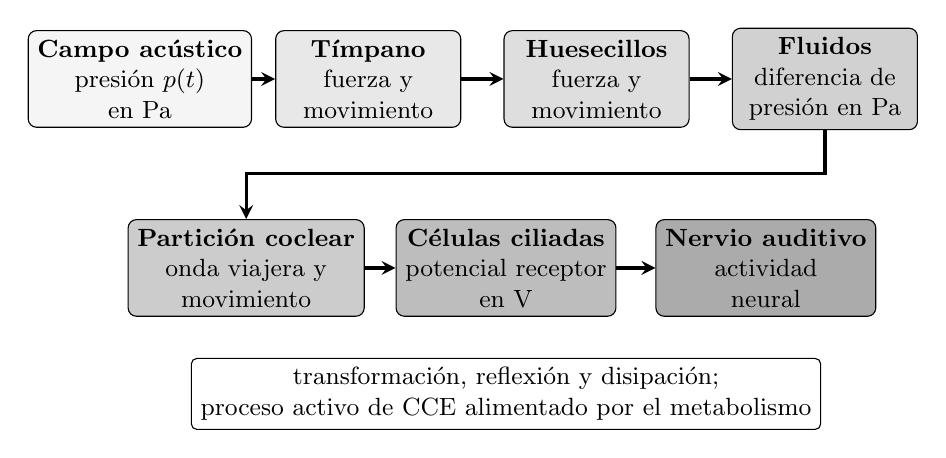
\begin{tikzpicture}[font=\small,>=stealth,x=1cm,y=1cm]
    \tikzset{
        stage/.style={
            draw,
            rounded corners=3pt,
            minimum width=2.35cm,
            minimum height=1.10cm,
            align=center
        },
        link/.style={->,very thick}
    }

    \node[stage,fill=black!4] (air) at (1.35,3.35)
        {\textbf{Campo acústico}\\presión \(p(t)\)\\en Pa};
    \node[stage,fill=black!9] (tm) at (4.25,3.35)
        {\textbf{Tímpano}\\fuerza y\\movimiento};
    \node[stage,fill=black!13] (oss) at (7.15,3.35)
        {\textbf{Huesecillos}\\fuerza y\\movimiento};
    \node[stage,fill=black!18] (fluid) at (10.05,3.35)
        {\textbf{Fluidos}\\diferencia de\\presión en Pa};

    \node[stage,fill=black!20] (partition) at (2.70,0.95)
        {\textbf{Partición coclear}\\onda viajera y\\movimiento};
    \node[stage,fill=black!26] (hair) at (6.00,0.95)
        {\textbf{Células ciliadas}\\potencial receptor\\en V};
    \node[stage,fill=black!33] (nerve) at (9.30,0.95)
        {\textbf{Nervio auditivo}\\actividad\\neural};

    \draw[link] (air.east) -- (tm.west);
    \draw[link] (tm.east) -- (oss.west);
    \draw[link] (oss.east) -- (fluid.west);
    \draw[link] (fluid.south) -- ++(0,-0.55) -| (partition.north);
    \draw[link] (partition.east) -- (hair.west);
    \draw[link] (hair.east) -- (nerve.west);

    \node[align=center,draw,rounded corners=2pt,fill=white] at (6.00,-0.65)
        {transformación, reflexión y disipación;\\
         proceso activo de CCE alimentado por el metabolismo};
\end{tikzpicture}

    \caption{Cadena funcional de la transducción auditiva periférica. La
    perturbación cambia de dominio físico a lo largo del recorrido: presión
    acústica, movimiento mecánico, presión y movimiento en fluidos, potencial
    receptor y actividad neural. El sombreado no representa niveles de energía
    ni magnitudes relativas. Esquema teórico, no anatómico y sin escala;
    elaboración propia.}
    \label{fig:sistema_auditivo}
\end{figure}

\section{Oído externo y membrana timpánica}
\label{sec:u6-oido-externo}

\subsection{Pabellón auricular}
\label{sec:u6-pabellon}

La geometría del pabellón y de la cabeza produce una respuesta
direccional dependiente de la frecuencia. Según la dirección de llegada,
algunas componentes se refuerzan y otras se atenúan; estas modificaciones
espectrales varían entre personas y aportan pistas para la localización~\cite{carlini2024}.
Aquí ``reforzar'' o ``atenuar'' describe un cambio físico de presión en el
canal respecto del campo incidente. No equivale todavía a un cambio fijo de
sonoridad, porque la sonoridad también depende de la señal, del oyente y del
contexto.

\subsection{Canal auditivo externo y frente de onda}
\label{sec:u6-cae}

El canal auditivo externo (CAE) conduce la perturbación hacia la membrana
timpánica. En el aire del canal existe movimiento local de partículas y se
superponen una onda que avanza hacia el tímpano con ondas reflejadas en las
terminaciones y en los cambios geométricos. Por eso, la presión acústica no es
idéntica en todos los puntos del CAE.

El CAE humano es curvo, posee sección variable y termina en una
membrana con impedancia finita. Su respuesta real no coincide exactamente con
la de un cilindro rígido y debe describirse mediante una función de
transferencia dependiente de la frecuencia y de la posición de medición~\cite{ugarteburu2022}.
Esta precisión resulta importante al diferenciar el nivel medido en el campo,
el nivel en la entrada del canal y el nivel próximo al tímpano.

\subsection{Modelo aproximado de cuarto de onda}
\label{sec:u6-modelo-cae}

Antes de estudiar la geometría real puede usarse un modelo simple. Se
representa el CAE como un tubo recto, abierto en la entrada y aproximadamente
cerrado en el extremo timpánico. Sean:

\begin{itemize}
    \item \(f_\mathrm{res}\), la primera frecuencia de resonancia, medida en
    hertz (\(\text{Hz}\));
    \item \(c\), la velocidad de propagación del sonido en el aire, medida en
    metros por segundo (\(\text{m}/\text{s}\));
    \item \(\ell\), la longitud efectiva del tubo, medida en metros
    (\(\text{m}\)).
\end{itemize}

En ese modelo ideal,

\begin{equation}
    f_\mathrm{res}\approx\frac{c}{4\ell}.
    \label{eq:u6-resonancia-cae}
\end{equation}

La igualdad no debe interpretarse como una medición anatómica exacta. Resume
la condición de cuarto de longitud de onda del modelo y omite curvatura,
variación de sección, pérdidas e impedancia del tímpano.

\subsection{Ejemplo resuelto: frecuencia del modelo de CAE}
\label{sec:u6-ejemplo-cae}

Se adopta, solo como dato didáctico, una longitud efectiva
\(\ell=27\,\text{mm}=0{,}027\,\text{m}\) y una velocidad de propagación
\(c=343\,\text{m}/\text{s}\). Entonces,

\[
    f_\mathrm{res}
      \approx\frac{343\,\text{m}/\text{s}}
                    {4(0{,}027\,\text{m})}
      \approx3176\,\text{Hz}
      \approx3{,}18\,\text{kHz}.
\]

Las unidades de longitud se cancelan y queda \(\text{s}^{-1}=\text{Hz}\).
El resultado pertenece al modelo ideal: no afirma que todas las personas
posean la misma frecuencia de resonancia ni que el cambio de nivel en el
tímpano sea universal.

\subsection{Membrana timpánica: de presión a fuerza distribuida}
\label{sec:u6-timpano}

La membrana timpánica separa el CAE de la cavidad del oído medio. Una
diferencia de presión entre sus caras produce una fuerza distribuida y una
deformación. Si se usa un modelo elemental con diferencia de presión
\(\Delta p\), medida en pascales (\(\text{Pa}\)), y un área efectiva \(A\),
medida en metros cuadrados (\(\text{m}^2\)), la magnitud de la fuerza
resultante \(F\), medida en newtons (\(\text{N}\)), se estima mediante

\begin{equation}
    F\approx\Delta p\,A.
    \label{eq:u6-fuerza-timpano}
\end{equation}

La membrana timpánica real es curva, no se desplaza como un pistón
rígido y presenta patrones de movimiento dependientes de la frecuencia. Su
acoplamiento con el mango del martillo transmite parte del movimiento al
sistema osicular~\cite{ugarteburu2022}. Por lo tanto, la ecuación~\eqref{eq:u6-fuerza-timpano}
sirve para interpretar la conversión presión--fuerza, no para predecir por sí
sola el movimiento completo del tímpano.

\section{Oído medio: transferencia y adaptación de impedancias}
\label{sec:u6-oido-medio}

\subsection{Caja timpánica, huesecillos, trompa y ventanas}
\label{sec:u6-anatomia-oido-medio}

El oído medio es una cavidad aérea que contiene la cadena formada por
martillo, yunque y estribo. El martillo se acopla a la membrana timpánica; el
estribo transmite movimiento a la ventana oval. La ventana redonda constituye
otra frontera móvil entre el oído medio y la cóclea~\cite{ugarteburu2022}.

La trompa de Eustaquio conecta funcionalmente la cavidad del oído
medio con la nasofaringe. Su apertura intermitente contribuye a equilibrar
presiones, ventilar y drenar el oído medio~\cite{schilder2015}. Si la presión estática a ambos
lados del tímpano difiere, cambia su posición de equilibrio y puede
modificarse la transferencia mecánica. Esta presión estática no debe
confundirse con la pequeña presión acústica alternante de una señal sonora.

La figura~\ref{fig:u6-organizacion-oido-periferico} ubica estas estructuras y
sus conexiones principales. Su geometría es esquemática: sirve para seguir el
recorrido funcional, no para medir dimensiones o ángulos anatómicos.

\begin{figure}[htbp]
    \centering
    % Propósito: ubicar las estructuras principales del oído externo, medio e
% interno y mostrar la continuidad de la vía aérea hasta la cóclea.
% Origen: descripción anatómica funcional de las secciones
% \ref{sec:u6-oido-externo}, \ref{sec:u6-anatomia-oido-medio} y
% \ref{sec:u6-rampas-fluidos}. Esquema propio, simplificado y sin escala.
% Descripción accesible: de izquierda a derecha se observan el pabellón y el
% canal auditivo externo, la membrana timpánica, los tres huesecillos, las
% ventanas oval y redonda y una cóclea en espiral. Una rama inferior representa
% la trompa de Eustaquio. Fondos grises separan oído externo, medio e interno.
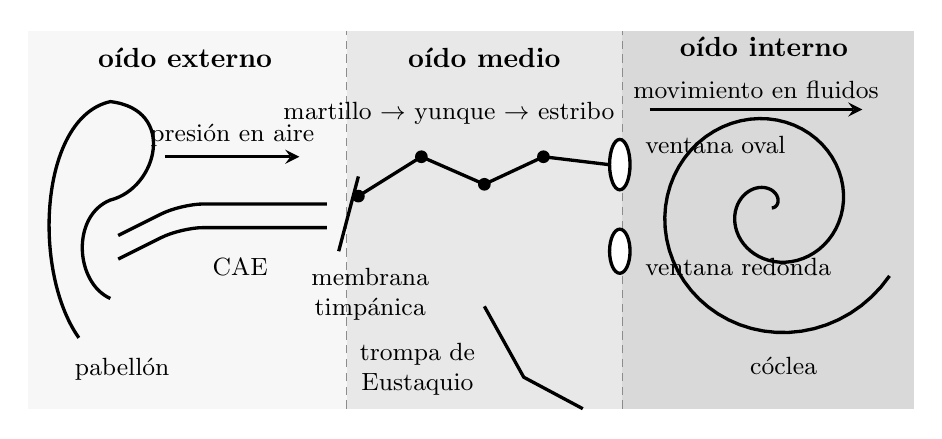
\begin{tikzpicture}[font=\small,>=stealth,x=1cm,y=1cm]
    \fill[black!3] (0.10,0.35) rectangle (4.15,5.15);
    \fill[black!9] (4.15,0.35) rectangle (7.65,5.15);
    \fill[black!15] (7.65,0.35) rectangle (11.35,5.15);
    \draw[densely dashed,black!45] (4.15,0.35) -- (4.15,5.15);
    \draw[densely dashed,black!45] (7.65,0.35) -- (7.65,5.15);

    \node[font=\bfseries] at (2.10,4.80) {oído externo};
    \node[font=\bfseries] at (5.90,4.80) {oído medio};
    \node[font=\bfseries] at (9.45,4.95) {oído interno};

    % Pabellón y canal auditivo externo.
    \draw[very thick]
        (0.75,1.25) .. controls (0.15,2.10) and (0.25,4.05) .. (1.15,4.25)
        .. controls (2.00,4.15) and (1.75,3.15) .. (1.15,3.00)
        .. controls (0.65,2.80) and (0.70,1.95) .. (1.15,1.75);
    \draw[very thick,rounded corners=8pt]
        (1.25,2.55) -- (2.05,2.95) -- (3.90,2.95);
    \draw[very thick,rounded corners=8pt]
        (1.25,2.25) -- (2.05,2.65) -- (3.90,2.65);
    \node[align=center] at (1.30,0.85) {pabellón};
    \node[align=center] at (2.80,2.15) {CAE};

    % Membrana timpánica y cadena osicular.
    \draw[very thick] (4.05,2.35) -- (4.30,3.30);
    \node[align=center] at (4.45,1.80) {membrana\\timpánica};
    \draw[very thick] (4.30,3.05) -- (5.10,3.55) -- (5.90,3.20)
        -- (6.65,3.55);
    \fill (4.30,3.05) circle (2.3pt);
    \fill (5.10,3.55) circle (2.3pt);
    \fill (5.90,3.20) circle (2.3pt);
    \fill (6.65,3.55) circle (2.3pt);
    \node[align=center] at (5.45,4.10) {martillo \(\rightarrow\) yunque
        \(\rightarrow\) estribo};
    \draw[very thick] (6.65,3.55) -- (7.48,3.45);

    % Ventanas, cóclea y trompa.
    \draw[very thick,fill=white] (7.62,3.45) ellipse (0.13 and 0.32);
    \draw[very thick,fill=white] (7.62,2.35) ellipse (0.13 and 0.28);
    \node[anchor=west] at (7.82,3.70) {ventana oval};
    \node[anchor=west] at (7.82,2.15) {ventana redonda};

    \draw[very thick]
        plot[domain=0:690,samples=120]
        ({9.55+0.0025*\x*cos(\x)},{2.90+0.0025*\x*sin(\x)});
    \node at (9.70,0.90) {cóclea};

    \draw[very thick] (5.90,1.65) -- (6.40,0.75) -- (7.15,0.35);
    \node[align=center] at (5.05,0.85) {trompa de\\Eustaquio};

    \draw[->,very thick] (1.85,3.55) -- (3.55,3.55)
        node[midway,above] {presión en aire};
    \draw[->,very thick] (8.00,4.15) -- (10.70,4.15)
        node[midway,above] {movimiento en fluidos};
\end{tikzpicture}

    \caption{Organización simplificada del oído periférico. La vía aérea
    atraviesa el pabellón y el CAE, mueve el tímpano y la cadena osicular, y
    alcanza la cóclea mediante la ventana oval; la ventana redonda aporta una
    frontera móvil complementaria. La trompa de Eustaquio comunica
    funcionalmente la caja timpánica con la nasofaringe. Esquema anatómico sin
    escala; elaboración propia.}
    \label{fig:u6-organizacion-oido-periferico}
\end{figure}

\subsection{Transformación de fuerza y desplazamiento}
\label{sec:u6-transformacion-oido-medio}

El paso del aire a los fluidos cocleares presenta una fuerte diferencia de
impedancias. Sin oído medio, una fracción importante de la energía incidente
se reflejaría en esa interfaz. El sistema timpánico--osicular contribuye a
adaptar la carga mediante dos recursos que pueden representarse de forma
ideal:

\begin{enumerate}
    \item una fuerza distribuida sobre un área timpánica efectiva se transmite
    hacia el área menor de la platina del estribo;
    \item la geometría del martillo y del yunque produce una acción de
    palanca.
\end{enumerate}

Sean \(A_\mathrm{TM}\) el área timpánica efectiva y \(A_\mathrm{E}\) el área
efectiva de la platina del estribo, ambas medidas en metros cuadrados
(\(\text{m}^2\)). Se define la razón de áreas adimensional

\begin{equation}
    R_A=\frac{A_\mathrm{TM}}{A_\mathrm{E}}.
    \label{eq:u6-razon-areas}
\end{equation}

Sea además \(R_L\) la razón de palanca, también adimensional, definida como la
razón ideal entre la fuerza de salida y la fuerza aplicada a la cadena. En un
modelo sin pérdidas, la razón de presiones \(R_p\) puede aproximarse por

\begin{equation}
    R_p\approx R_A R_L.
    \label{eq:u6-razon-presiones}
\end{equation}

Este aumento de presión no implica aumento de energía. En un transformador
ideal, una mayor fuerza de salida se acompaña por menor desplazamiento o
velocidad en la salida. En el oído real, la elasticidad, la masa, el
amortiguamiento y la carga coclear vuelven la transferencia dependiente de la
frecuencia.

\subsection{Ejemplo resuelto: transformación ideal de presión}
\label{sec:u6-ejemplo-oido-medio}

Para practicar el modelo, se adoptan las razones didácticas \(R_A=20\) y
\(R_L=1{,}2\). No se las presenta como dimensiones anatómicas universales.
La razón ideal de presiones es

\[
    R_p\approx20(1{,}2)=24.
\]

Si se desea expresar esa razón de amplitudes de presión mediante un nivel
\(G_p\), medido en decibeles (\(\text{dB}\)), se define

\begin{equation}
    G_p=20\log_{10}(R_p).
    \label{eq:u6-nivel-transformacion-presion}
\end{equation}

Por lo tanto,

\[
    G_p=20\log_{10}(24)\approx27{,}60\,\text{dB}.
\]

El resultado significa que el modelo ideal entrega una presión 24 veces mayor
en la salida que en la entrada elegida. No es un nivel de presión sonora en
dB SPL, no es una ganancia de energía y no representa por sí solo la función
de transferencia medida del oído medio.

La figura~\ref{fig:u6-adaptacion-oido-medio} reúne la relación de áreas y la
acción de palanca. Debe leerse como un transformador mecánico ideal, no como
una representación exacta de la geometría osicular. En ella,
\(\Delta p_\mathrm{TM}\) es la amplitud de la diferencia de presión sobre el
tímpano y \(p_\mathrm{E}\) es la amplitud de presión a la salida del modelo,
ambas medidas en pascales (\(\text{Pa}\)).

\begin{figure}[htbp]
    \centering
    % Propósito: mostrar cómo la relación de áreas y la palanca aumentan la razón
% de presiones mientras disminuyen desplazamiento o velocidad en el modelo
% ideal, sin aumento de energía.
% Origen: F=Delta p A, R_A=A_TM/A_E, F_E/F_TM=R_L y
% R_p=p_E/Delta p_TM aproximadamente igual a R_A R_L; ecuaciones
% \eqref{eq:u6-fuerza-timpano}--\eqref{eq:u6-razon-presiones}.
% Descripción accesible: una presión actúa sobre el área timpánica grande y
% produce una fuerza. Una palanca representa martillo y yunque. La fuerza llega
% a la platina pequeña del estribo, donde la razón de presiones aumenta. Debajo
% se indica que mayor presión y fuerza se acompañan por menor velocidad o
% desplazamiento y que el modelo no crea energía.
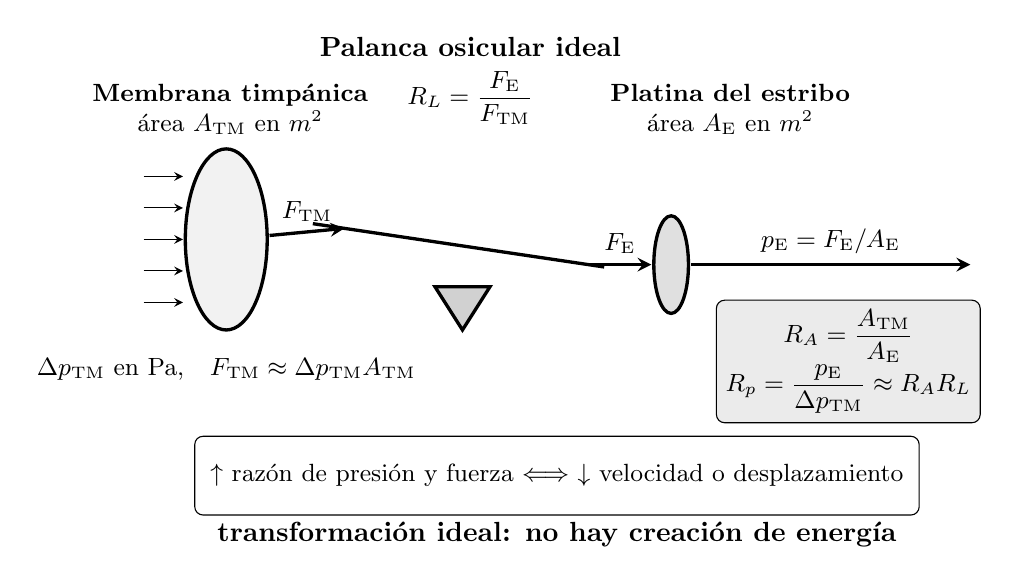
\begin{tikzpicture}[font=\small,>=stealth,x=1cm,y=1cm]
    \tikzset{
        box/.style={draw,rounded corners=3pt,align=center,minimum height=1.0cm},
        flow/.style={->,very thick}
    }

    \draw[very thick,fill=black!5] (1.15,1.90) ellipse (0.52 and 1.15);
    \foreach \yy in {1.10,1.50,1.90,2.30,2.70}{
        \draw[->] (0.10,\yy) -- (0.60,\yy);
    }
    \node[align=center] at (1.20,3.55)
        {\textbf{Membrana timpánica}\\
         área \(A_\mathrm{TM}\) en \(\text{m}^2\)};
    \node[align=center] at (1.15,0.25)
        {\(\Delta p_\mathrm{TM}\) en Pa,\quad
         \(F_\mathrm{TM}\approx\Delta p_\mathrm{TM}A_\mathrm{TM}\)};

    % Palanca ideal.
    \draw[very thick] (2.25,2.10) -- (5.95,1.55);
    \draw[very thick,fill=black!18] (4.15,0.75) -- (3.80,1.30)
        -- (4.50,1.30) -- cycle;
    \draw[flow] (1.70,1.95) -- (2.65,2.04)
        node[midway,above] {\(F_\mathrm{TM}\)};
    \draw[flow] (5.75,1.58) -- (6.55,1.58)
        node[midway,above] {\(F_\mathrm{E}\)};
    \node[font=\bfseries] at (4.25,4.35)
        {Palanca osicular ideal};
    \node at (4.25,3.70)
        {\(\displaystyle R_L=\frac{F_\mathrm{E}}{F_\mathrm{TM}}\)};

    % Platina del estribo.
    \draw[very thick,fill=black!12] (6.80,1.58) ellipse (0.22 and 0.62);
    \node[align=center] at (7.55,3.55)
        {\textbf{Platina del estribo}\\
         área \(A_\mathrm{E}\) en \(\text{m}^2\)};
    \draw[flow] (7.05,1.58) -- (10.60,1.58)
        node[midway,above] {\(p_\mathrm{E}=F_\mathrm{E}/A_\mathrm{E}\)};
    \node[box,fill=black!8,minimum width=3.25cm] at (9.05,0.35)
        {\(\displaystyle R_A=\frac{A_\mathrm{TM}}{A_\mathrm{E}}\)\\
         \(\displaystyle R_p=\frac{p_\mathrm{E}}{\Delta p_\mathrm{TM}}
             \approx R_A R_L\)};

    \node[box,fill=white,minimum width=9.20cm] at (5.35,-1.10)
        {\(\uparrow\) razón de presión y fuerza
         \(\Longleftrightarrow\)
         \(\downarrow\) velocidad o desplazamiento};
    \node[font=\bfseries] at (5.35,-1.85)
        {transformación ideal: no hay creación de energía};
\end{tikzpicture}

    \caption{Adaptación de impedancias en el modelo ideal del oído medio. La
    presión sobre el área timpánica efectiva produce una fuerza que se
    transmite mediante la palanca osicular hacia el área menor de la platina
    del estribo. El aumento de la razón de presiones se acompaña por una
    reducción de velocidad o desplazamiento y no implica creación de energía.
    Las áreas y longitudes dibujadas no están a escala; elaboración propia.}
    \label{fig:u6-adaptacion-oido-medio}
\end{figure}

\subsection{Reflejo acústico del estapedio}
\label{sec:u6-reflejo-estapedial}

Ante determinados estímulos sonoros de nivel elevado, una vía refleja
produce la contracción del músculo estapedio. La contracción modifica la
rigidez de la cadena y atenúa su transferencia de manera dependiente de la
frecuencia, con efecto más marcado en frecuencias bajas. El umbral y la
latencia dependen del estímulo, del nivel y de la persona; la latencia
disminuye cuando aumenta el nivel por encima del umbral~\cite{ashaHearingAdults}.

No corresponde fijar un único umbral en dB SPL ni una única latencia para
todos los casos. El reflejo no puede proteger frente al comienzo de un impulso
que llega antes de que se complete la respuesta muscular, y tampoco debe
presentarse como una protección absoluta frente a niveles peligrosos.

El cambio de inmitancia asociado con el reflejo puede medirse con
instrumentación audiológica. Su presencia, ausencia o umbral aporta
información sobre varias partes del sistema, pero no identifica por sí solo
una etiología~\cite{ashaHearingAdults}. La interpretación diagnóstica y los protocolos de medición se
reservan para la Unidad~\ref{chap:unidad-8}.

\section{Audición por conducción ósea}
\label{sec:u6-conduccion-osea}

En la vía aérea, la perturbación llega principalmente por el CAE, el tímpano y
la cadena osicular. En la conducción ósea, una fuerza variable aplicada al
cráneo o a los tejidos produce vibraciones que alcanzan la cóclea mediante
varios mecanismos. No existe un nivel único a partir del cual ``aparezca'' la
conducción ósea, ni resulta adecuado describir cualquier estímulo óseo solo
mediante dB SPL.

En una descripción funcional pueden distinguirse al menos las
siguientes contribuciones, que actúan simultáneamente y cuya importancia
relativa depende de la frecuencia, el punto de estimulación y el
acoplamiento~\cite{stenfeltGoode2005}:

\begin{enumerate}
    \item \textbf{Radiación hacia el CAE:} la vibración de sus paredes
    produce presión acústica en el aire del canal; la oclusión puede modificar
    esta contribución~\cite{stenfeltGoode2005}.
    \item \textbf{Inercia de los huesecillos:} el movimiento relativo
    entre la cadena osicular y las paredes de la cavidad puede desplazar el
    estribo~\cite{stenfeltGoode2005}.
    \item \textbf{Inercia de los fluidos cocleares:} el movimiento del
    cráneo puede producir movimiento relativo de los fluidos respecto de la
    cápsula~\cite{stenfeltGoode2005}.
    \item \textbf{Deformación de la cápsula coclear:} cambios pequeños
    de forma pueden generar diferencias de presión entre compartimentos~\cite{stenfeltGoode2005}.
    \item \textbf{Transmisión por tejidos y cavidades:} otras rutas,
    incluida la comunicación con fluidos intracraneales, pueden contribuir al
    movimiento coclear~\cite{stenfeltGoode2005}.
\end{enumerate}

Estas contribuciones convergen en un resultado: generar diferencias de
presión y movimiento relativo en la partición coclear. Por eso, afirmar que la
vía ósea ``evita por completo'' el oído externo y medio también es una
simplificación.

La figura~\ref{fig:u6-conduccion-osea} representa la convergencia de los
mecanismos sin asignarles una importancia fija.

\begin{figure}[htbp]
    \centering
    % Propósito: evitar la representación de la conducción ósea como una única
% ruta que omite por completo el oído externo y el medio.
% Origen: cinco contribuciones funcionales enumeradas en la sección
% \ref{sec:u6-conduccion-osea}. Esquema conceptual; no expresa magnitudes ni
% importancia relativa.
% Descripción accesible: una vibración aplicada al cráneo o a los tejidos se
% divide en cinco rutas paralelas: radiación hacia el canal, inercia osicular,
% inercia de fluidos, deformación de la cápsula y transmisión por tejidos y
% cavidades. Todas convergen en diferencias de presión y movimiento de la
% partición coclear. Una nota aclara que actúan simultáneamente y con peso
% dependiente de frecuencia, punto de estimulación y acoplamiento.
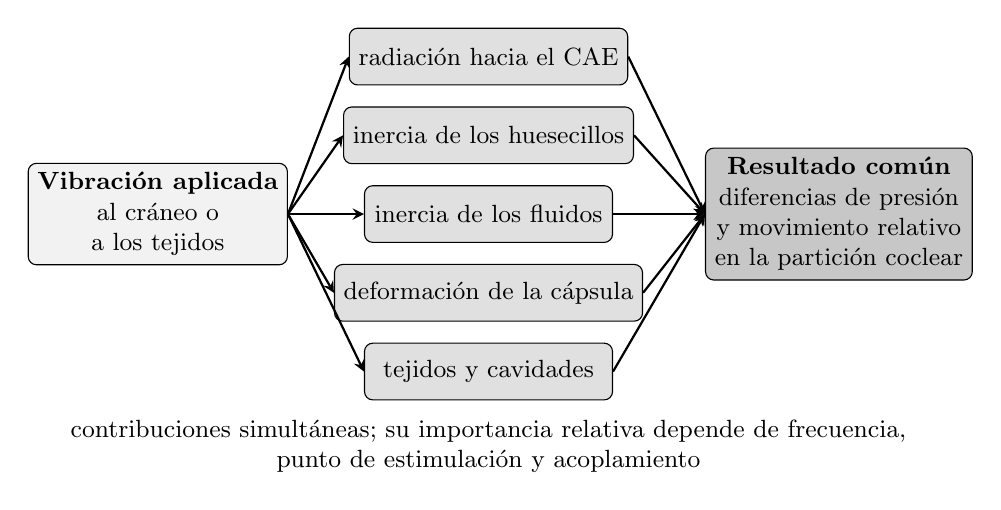
\begin{tikzpicture}[font=\small,>=stealth,x=1cm,y=1cm]
    \tikzset{
        source/.style={
            draw,rounded corners=3pt,fill=black!5,
            minimum width=2.45cm,minimum height=1.25cm,align=center
        },
        route/.style={
            draw,rounded corners=3pt,fill=black!12,
            minimum width=3.15cm,minimum height=0.72cm,align=center
        },
        result/.style={
            draw,rounded corners=3pt,fill=black!22,
            minimum width=2.65cm,minimum height=1.45cm,align=center
        },
        flow/.style={->,thick}
    }

    \node[source] (input) at (1.35,2.75)
        {\textbf{Vibración aplicada}\\al cráneo o\\a los tejidos};

    \node[route] (cae) at (5.55,4.75) {radiación hacia el CAE};
    \node[route] (oss) at (5.55,3.75) {inercia de los huesecillos};
    \node[route] (fluid) at (5.55,2.75) {inercia de los fluidos};
    \node[route] (capsule) at (5.55,1.75) {deformación de la cápsula};
    \node[route] (tissue) at (5.55,0.75) {tejidos y cavidades};

    \node[result] (output) at (10.00,2.75)
        {\textbf{Resultado común}\\diferencias de presión\\y movimiento relativo\\
         en la partición coclear};

    \foreach \n in {cae,oss,fluid,capsule,tissue}{
        \draw[flow] (input.east) -- (\n.west);
        \draw[flow] (\n.east) -- (output.west);
    }

    \node[align=center] at (5.55,-0.20)
        {contribuciones simultáneas; su importancia relativa depende de
         frecuencia,\\punto de estimulación y acoplamiento};
\end{tikzpicture}

    \caption{Conducción ósea como resultado de varias contribuciones
    simultáneas. La radiación hacia el CAE, las inercias osicular y de fluidos,
    la deformación de la cápsula y otras rutas por tejidos y cavidades pueden
    contribuir al movimiento coclear. El esquema no establece una ruta única
    ni cuantifica su importancia relativa; elaboración propia.}
    \label{fig:u6-conduccion-osea}
\end{figure}

\section{Oído interno: arquitectura y mecánica coclear}
\label{sec:u6-oido-interno}

\subsection{Rampas, fluidos y membranas}
\label{sec:u6-rampas-fluidos}

La cóclea contiene tres compartimentos longitudinales: rampa
vestibular, conducto coclear o rampa media y rampa timpánica. Las rampas
vestibular y timpánica contienen perilinfa y se comunican en la región apical
mediante el helicotrema; la rampa media contiene endolinfa~\cite{fettiplace2017}.

La membrana de Reissner separa la rampa vestibular de la rampa media.
La membrana basilar y el órgano de Corti forman parte de la separación entre
la rampa media y la rampa timpánica. La membrana tectorial se ubica sobre los
haces de estereocilios del órgano de Corti y participa en su micromecánica~\cite{fettiplace2017}.

El movimiento del estribo en la ventana oval produce variaciones de presión
en los fluidos. Como los líquidos son poco compresibles, la ventana redonda
proporciona una frontera móvil complementaria. No debe imaginarse un flujo
continuo desde la ventana oval hasta la redonda: durante una señal sonora los
movimientos son oscilatorios y las partículas se desplazan alrededor de una
posición de equilibrio.

La figura~\ref{fig:u6-arquitectura-coclear} combina dos vistas necesarias:
una vista longitudinal para las ventanas y el helicotrema, y un corte
transversal para las rampas y membranas.

\begin{figure}[htbp]
    \centering
    % Propósito: relacionar el recorrido longitudinal entre las ventanas y el
% helicotrema con la organización transversal de rampas, fluidos y membranas.
% Origen: descripción de la sección \ref{sec:u6-rampas-fluidos}. Esquema
% anatómico propio, simplificado y sin escala.
% Descripción accesible: el panel izquierdo muestra una cóclea desenrollada.
% La rampa vestibular parte de la ventana oval, se comunica con la rampa
% timpánica en el helicotrema y esta termina en la ventana redonda; la rampa
% media queda entre ambas. El panel derecho muestra un corte transversal con
% perilinfa arriba y abajo, endolinfa en la rampa media, membrana de Reissner,
% membrana basilar, membrana tectorial y órgano de Corti.
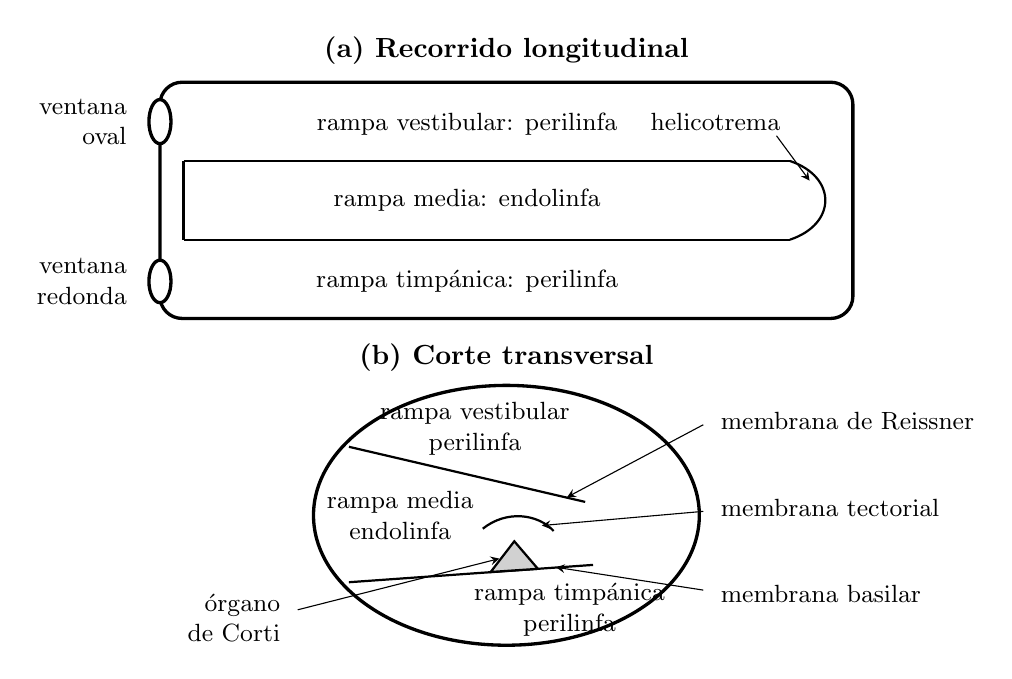
\begin{tikzpicture}[font=\small,>=stealth,x=1cm,y=1cm]
    % Panel longitudinal apilado: las tres rampas ocupan bandas separadas;
    % las ventanas se ubican en la base y el helicotrema en el extremo apical.
    \node[font=\bfseries] at (5.85,7.75) {(a) Recorrido longitudinal};
    \draw[very thick,rounded corners=8pt] (1.45,4.35) rectangle (10.25,7.35);
    \draw[thick] (1.75,6.35) -- (9.45,6.35);
    \draw[thick] (1.75,5.35) -- (9.45,5.35);
    \draw[thick] (9.45,6.35) .. controls (10.05,6.15) and (10.05,5.55) ..
        (9.45,5.35);
    \draw[thick] (1.75,6.35) -- (1.75,5.35);

    \node[align=center] at (5.35,6.82) {rampa vestibular: perilinfa};
    \node[align=center] at (5.35,5.85) {rampa media: endolinfa};
    \node[align=center] at (5.35,4.82) {rampa timpánica: perilinfa};

    \node[anchor=east] at (9.45,6.85) {helicotrema};
    \draw[->] (9.28,6.67) -- (9.70,6.10);

    \draw[very thick,fill=white] (1.45,6.85) ellipse (0.14 and 0.28);
    \draw[very thick,fill=white] (1.45,4.82) ellipse (0.14 and 0.27);
    \node[anchor=east,align=right] at (1.15,6.85) {ventana\\oval};
    \node[anchor=east,align=right] at (1.15,4.82) {ventana\\redonda};

    % Panel transversal apilado: las rampas se rotulan dentro del corte y las
    % llamadas de las membranas se ordenan en una columna exterior.
    \node[font=\bfseries] at (5.85,3.85) {(b) Corte transversal};
    \draw[very thick] (5.85,1.85) ellipse (2.45 and 1.65);
    \draw[thick] (3.85,2.72) -- (6.85,2.02);
    \draw[thick] (3.85,1.00) -- (6.95,1.22);

    \node[align=center] at (5.45,2.95)
        {rampa vestibular\\perilinfa};
    \node[align=center] at (4.50,1.85)
        {rampa media\\endolinfa};
    \node[align=center] at (6.65,0.65)
        {rampa timpánica\\perilinfa};

    \node[anchor=west,align=left] at (8.45,3.05)
        {membrana de Reissner};
    \draw[->] (8.35,3.00) -- (6.62,2.08);

    \draw[thick,fill=black!18] (5.65,1.13) -- (5.95,1.52)
        -- (6.25,1.17) -- cycle;
    \draw[thick] (5.55,1.68) .. controls (5.85,1.92) and (6.25,1.87) ..
        (6.45,1.65);

    \node[anchor=west,align=left] at (8.45,1.95)
        {membrana tectorial};
    \draw[->] (8.35,1.90) -- (6.30,1.72);

    \node[anchor=west,align=left] at (8.45,0.85)
        {membrana basilar};
    \draw[->] (8.35,0.90) -- (6.48,1.19);

    \node[anchor=east,align=right] at (3.10,0.55) {órgano\\de Corti};
    \draw[->] (3.20,0.65) -- (5.76,1.30);
\end{tikzpicture}

    \caption{Arquitectura coclear simplificada. (a)~Vista longitudinal
    desenrollada: la rampa vestibular comienza en la ventana oval, se comunica
    con la rampa timpánica mediante el helicotrema y esta última termina en la
    ventana redonda. (b)~Corte transversal: la membrana de Reissner y la
    membrana basilar delimitan la rampa media; el órgano de Corti se apoya
    sobre la membrana basilar y se relaciona con la membrana tectorial. Esquema
    sin escala; elaboración propia.}
    \label{fig:u6-arquitectura-coclear}
\end{figure}

\subsection{Onda viajera y lugar característico}
\label{sec:u6-onda-viajera}

Una estimulación tonal produce una onda viajera en la partición
coclear. La onda comienza en la región basal, aumenta progresivamente y
alcanza un máximo en una región dependiente de la frecuencia antes de
decaer. Las frecuencias altas alcanzan su máximo más cerca de la base; las
frecuencias bajas, en regiones más apicales~\cite{fettiplace2017,capraraPeng2022}.

La ubicación de máxima respuesta se denomina \textbf{lugar característico}.
La organización ordenada de frecuencias a lo largo de la cóclea se denomina
\textbf{tonotopía}. Esto no significa que un tono active un segmento de ancho
fijo ni que la cóclea ejecute una transformada rápida de Fourier literal. La
respuesta posee extensión espacial, solapamiento entre frecuencias y
dependencia con el nivel.

La variación longitudinal de rigidez, dimensiones y carga de la
partición coclear contribuye a la tonotopía, pero la selectividad de la cóclea
viva también depende de la interacción con los fluidos y de procesos activos
asociados con las células ciliadas externas~\cite{fettiplace2017,capraraPeng2022}.

\subsection{Señales débiles e intensas}
\label{sec:u6-debiles-intensas}

Para señales débiles, el proceso activo coclear aumenta localmente la
sensibilidad y agudiza la selectividad cerca del lugar característico. A
medida que aumenta el nivel de la señal, esa contribución activa no crece en
la misma proporción: la respuesta es compresiva y la región excitada tiende a
ensancharse~\cite{fettiplace2017,capraraPeng2022}.

Por lo tanto, no existe una ganancia coclear única aplicable a cualquier
frecuencia y nivel. ``Amplificador coclear'' es el nombre de un proceso activo
y no de un bloque electrónico con ganancia constante. Esta no linealidad
contribuye a representar un intervalo amplio de niveles, pero la experiencia
de sonoridad requiere procesamiento adicional y se estudiará en la
Unidad~\ref{chap:unidad-7}.

La figura~\ref{fig:u6-onda-viajera-tonotopia} muestra por separado la
dependencia con la frecuencia y la dependencia con el nivel.

\begin{figure}[htbp]
    \centering
    % Propósito: mostrar que el máximo de la onda viajera depende de la frecuencia
% y que la extensión espacial también depende del nivel.
% Origen: envolventes analíticas esquemáticas
% y(s)=C(s/s_c)^a exp[a(1-s/s_c)], con 0<=s<=1 y C elegido para fijar
% la escala vertical indicada. En el panel (a),
% a=3 y s_c={0,20; 0,50; 0,80}; cada curva se normaliza a su máximo.
% En el panel (b), s_c=0,55 y se comparan una envolvente estrecha (a=8,
% escala 0,62) y otra más ancha (a=3, escala 1,00). Los parámetros son
% didácticos y no representan datos anatómicos o experimentales.
% Descripción accesible: en el panel superior, tres ondas parten de la base.
% La frecuencia alta alcanza su máximo cerca de la base, la media en la zona
% central y la baja cerca del ápice. En el panel inferior, para una misma
% frecuencia, la señal débil produce una respuesta más estrecha y menor en la
% escala esquemática; la intensa produce una respuesta mayor y más extendida.
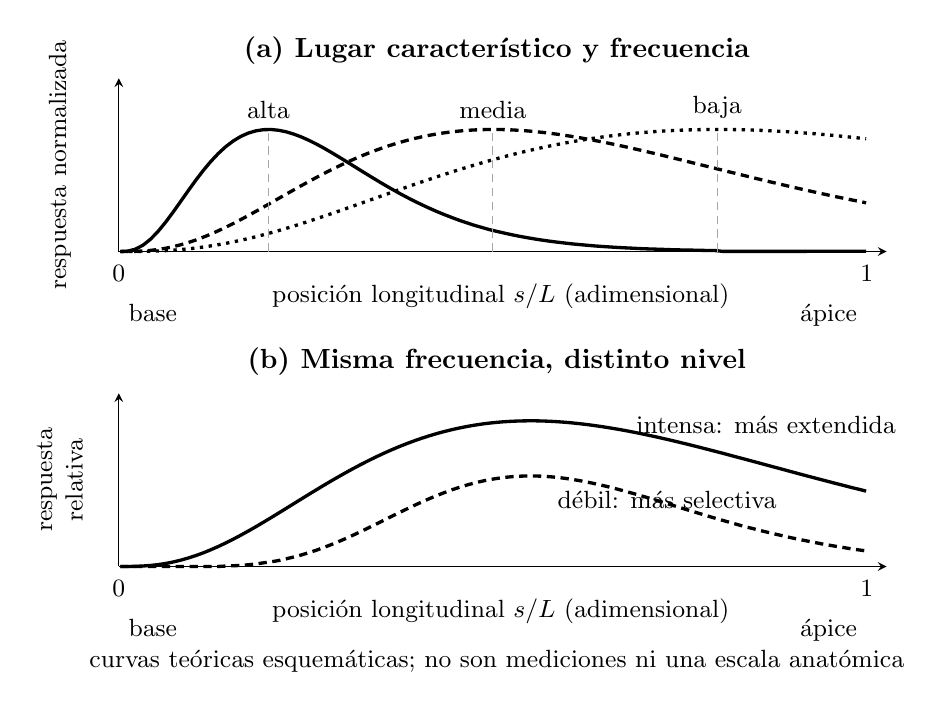
\begin{tikzpicture}[font=\small,>=stealth,x=1cm,y=1cm]
    % Panel (a): tonotopía.
    \node[font=\bfseries] at (5.90,6.20)
        {(a) Lugar característico y frecuencia};
    \draw[->] (1.10,3.65) -- (10.85,3.65);
    \draw[->] (1.10,3.65) -- (1.10,5.85);
    \node[rotate=90] at (0.35,4.75) {respuesta normalizada};
    \node at (5.95,3.08)
        {posición longitudinal \(s/L\) (adimensional)};
    \node[anchor=north] at (1.10,3.60) {\(0\)};
    \node[anchor=north] at (10.60,3.60) {\(1\)};
    \node[anchor=north west] at (1.10,3.10) {base};
    \node[anchor=north east] at (10.60,3.10) {ápice};

    \draw[very thick,samples=100,domain=0.002:1]
        plot ({1.10+9.50*\x},
        {3.65+1.55*pow(\x/0.20,3)*exp(3*(1-\x/0.20))});
    \draw[very thick,densely dashed,samples=100,domain=0.002:1]
        plot ({1.10+9.50*\x},
        {3.65+1.55*pow(\x/0.50,3)*exp(3*(1-\x/0.50))});
    \draw[very thick,dotted,samples=100,domain=0.002:1]
        plot ({1.10+9.50*\x},
        {3.65+1.55*pow(\x/0.80,3)*exp(3*(1-\x/0.80))});

    \draw[densely dashed,black!35] (3.00,3.65) -- (3.00,5.20);
    \draw[densely dashed,black!35] (5.85,3.65) -- (5.85,5.20);
    \draw[densely dashed,black!35] (8.70,3.65) -- (8.70,5.20);
    \node[anchor=south] at (3.00,5.22) {alta};
    \node[anchor=south] at (5.85,5.22) {media};
    \node[anchor=south] at (8.70,5.22) {baja};

    % Panel (b): dependencia del nivel.
    \node[font=\bfseries] at (5.90,2.25)
        {(b) Misma frecuencia, distinto nivel};
    \draw[->] (1.10,-0.35) -- (10.85,-0.35);
    \draw[->] (1.10,-0.35) -- (1.10,1.85);
    \node[rotate=90,align=center] at (0.35,0.75)
        {respuesta\\relativa};
    \node at (5.95,-0.92)
        {posición longitudinal \(s/L\) (adimensional)};
    \node[anchor=north] at (1.10,-0.40) {\(0\)};
    \node[anchor=north] at (10.60,-0.40) {\(1\)};
    \node[anchor=north west] at (1.10,-0.90) {base};
    \node[anchor=north east] at (10.60,-0.90) {ápice};

    \draw[very thick,densely dashed,samples=100,domain=0.002:1]
        plot ({1.10+9.50*\x},
        {-0.35+1.15*pow(\x/0.55,8)*exp(8*(1-\x/0.55))});
    \draw[very thick,samples=100,domain=0.002:1]
        plot ({1.10+9.50*\x},
        {-0.35+1.85*pow(\x/0.55,3)*exp(3*(1-\x/0.55))});
    \node[anchor=west] at (7.55,1.45) {intensa: más extendida};
    \node[anchor=west] at (6.55,0.50) {débil: más selectiva};
    \node[align=center] at (5.90,-1.55)
        {curvas teóricas esquemáticas; no son mediciones ni una escala anatómica};
\end{tikzpicture}

    \caption{Envolventes teóricas de la onda viajera. (a)~En la coordenada
    longitudinal normalizada \(s/L\), las frecuencias altas alcanzan su máximo
    cerca de la base y las bajas más cerca del ápice. (b)~Para una misma
    frecuencia, la respuesta ante una señal intensa se representa con mayor
    amplitud y extensión espacial que la respuesta selectiva ante una señal
    débil. Las curvas se construyeron con funciones analíticas normalizadas y
    parámetros didácticos: no son datos experimentales ni una escala
    anatómica; elaboración propia.}
    \label{fig:u6-onda-viajera-tonotopia}
\end{figure}

\section{Órgano de Corti y células ciliadas}
\label{sec:u6-organo-corti}

\subsection{Micromecánica del órgano de Corti}
\label{sec:u6-micromecanica}

El órgano de Corti se apoya sobre la membrana basilar y contiene
células de sostén, una fila de células ciliadas internas (CCI) y varias filas
de células ciliadas externas (CCE). El movimiento relativo entre membrana
basilar, membrana tectorial y otras estructuras de la partición produce
deflexión de los haces de estereocilios~\cite{fettiplace2017,capraraPeng2022}.

La membrana basilar no actúa sola: el estímulo relevante para las células
ciliadas depende del movimiento relativo dentro de la partición. Esta
distinción evita imaginar la cóclea como una hilera de resonadores pasivos
independientes.

\subsection{Funciones diferenciadas de CCI y CCE}
\label{sec:u6-cci-cce}

\textbf{Células ciliadas internas.} Las CCI constituyen la vía
sensorial aferente principal. Sus potenciales receptores regulan la liberación
de glutamato en sinapsis especializadas con la gran mayoría de las fibras
aferentes del ganglio espiral~\cite{fettiplace2017,capraraPeng2022}.

\textbf{Células ciliadas externas.} Las CCE cambian su longitud en
respuesta a variaciones de potencial mediante un mecanismo asociado con la
proteína prestina. Su acción mecánica realimenta localmente la partición
coclear y contribuye a la sensibilidad, la compresión y la selectividad
frecuencial, especialmente para señales débiles~\cite{fettiplace2017,capraraPeng2022}.

Ambos tipos celulares realizan transducción mecanoeléctrica, pero no cumplen
la misma función global. No debe atribuirse a las CCE la transmisión aferente
principal ni reducirse las CCI a un papel pasivo.

\subsection{Secuencia de transducción mecanoeléctrica}
\label{sec:u6-transduccion}

Los estereocilios se organizan en haces polarizados y se conectan
mediante enlaces apicales o \emph{tip links}. La deflexión hacia la dirección
excitatoria aumenta la tensión sobre esos enlaces y eleva la probabilidad de
apertura de canales de transducción mecanosensibles; la deflexión opuesta la
reduce. Los enlaces no son los canales~\cite{fettiplace2017,capraraPeng2022}.

La endolinfa posee una composición iónica y un potencial eléctrico
que favorecen la entrada de cationes, principalmente potasio
\(\text{K}^{+}\), cuando se abren los canales. La corriente modifica de forma
graduada el potencial de membrana de la célula. No existe un desplazamiento
único que funcione como umbral mecánico de todo o nada~\cite{fettiplace2017,capraraPeng2022}.

En una CCI, la despolarización abre canales de calcio
\(\text{Ca}^{2+}\) dependientes de voltaje en la región basal. La entrada de
calcio regula la liberación de glutamato en las sinapsis de cinta; el
neurotransmisor modifica la probabilidad de descarga de las fibras
aferentes~\cite{fettiplace2017,capraraPeng2022}.

La secuencia puede resumirse así:

\[
\begin{aligned}
\text{movimiento relativo}
&\longrightarrow \text{deflexión del haz}\\
&\longrightarrow \text{cambio de apertura de canales}\\
&\longrightarrow \text{potencial receptor graduado}\\
&\longrightarrow \text{liberación de neurotransmisor}\\
&\longrightarrow \text{actividad neural}.
\end{aligned}
\]

Una señal eléctrica celular no es todavía un potencial de acción del nervio.
La célula ciliada produce un potencial receptor graduado; las fibras
aferentes generan potenciales de acción.

La figura~\ref{fig:u6-funciones-cci-cce} integra el paso de transducción común
con las consecuencias funcionales diferenciadas.

\begin{figure}[!htbp]
    \centering
    % Propósito: distinguir la función aferente principal de las CCI de la
% realimentación mecánica activa aportada por las CCE.
% Origen: secciones \ref{sec:u6-micromecanica},
% \ref{sec:u6-cci-cce} y \ref{sec:u6-transduccion}. Diagrama funcional; no
% representa cantidades celulares, proporciones anatómicas ni conexiones
% individuales.
% Descripción accesible: el movimiento relativo de la partición deflecta los
% estereocilios y produce un potencial receptor en ambos tipos celulares. La
% rama izquierda muestra que las células ciliadas internas liberan glutamato
% hacia la vía aferente principal. La rama derecha muestra que las células
% ciliadas externas cambian de longitud y realimentan la mecánica coclear,
% modificando sensibilidad y selectividad. Una flecha de retorno representa
% esa realimentación.
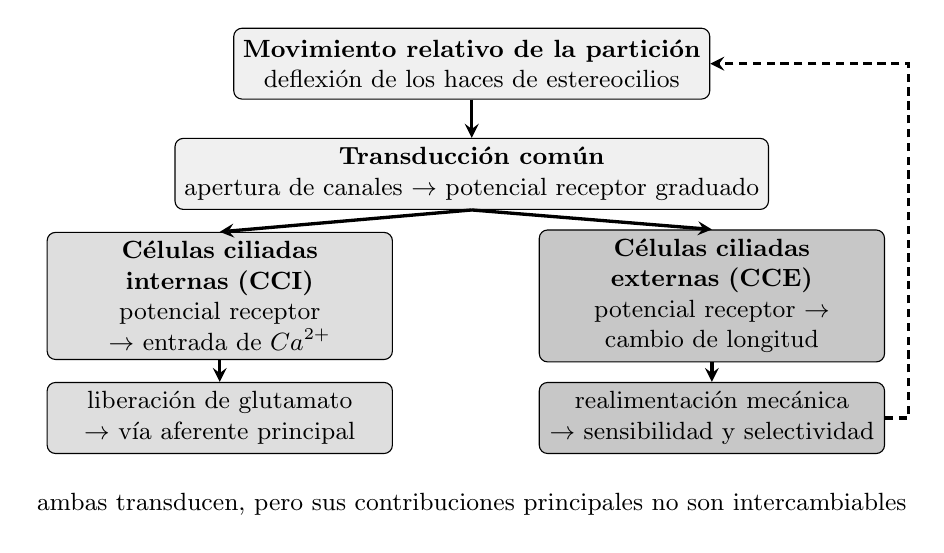
\begin{tikzpicture}[font=\small,>=stealth,x=1cm,y=1cm]
    \tikzset{
        common/.style={
            draw,rounded corners=3pt,fill=black!6,
            minimum width=4.30cm,minimum height=0.90cm,align=center
        },
        cci/.style={
            draw,rounded corners=3pt,fill=black!13,
            text width=4.15cm,minimum height=0.90cm,align=center
        },
        cce/.style={
            draw,rounded corners=3pt,fill=black!22,
            text width=4.15cm,minimum height=0.90cm,align=center
        },
        flow/.style={->,very thick}
    }

    \node[common] (motion) at (5.75,5.05)
        {\textbf{Movimiento relativo de la partición}\\
         deflexión de los haces de estereocilios};
    \node[common] (met) at (5.75,3.65)
        {\textbf{Transducción común}\\
         apertura de canales \(\rightarrow\) potencial receptor graduado};
    \draw[flow] (motion.south) -- (met.north);

    \node[cci] (ci) at (2.55,2.10)
        {\textbf{Células ciliadas internas (CCI)}\\
         potencial receptor \(\rightarrow\) entrada de \(\text{Ca}^{2+}\)};
    \node[cce] (ce) at (8.80,2.10)
        {\textbf{Células ciliadas externas (CCE)}\\
         potencial receptor \(\rightarrow\) cambio de longitud};
    \draw[flow] (met.south) -- (ci.north);
    \draw[flow] (met.south) -- (ce.north);

    \node[cci] (afferent) at (2.55,0.55)
        {liberación de glutamato\\
         \(\rightarrow\) vía aferente principal};
    \node[cce] (feedback) at (8.80,0.55)
        {realimentación mecánica\\
         \(\rightarrow\) sensibilidad y selectividad};
    \draw[flow] (ci.south) -- (afferent.north);
    \draw[flow] (ce.south) -- (feedback.north);

    \draw[->,very thick,densely dashed] (feedback.east) -- (11.30,0.55)
        -- (11.30,5.05) -- (motion.east);

    \node[align=center] at (5.75,-0.55)
        {ambas transducen, pero sus contribuciones principales no son
         intercambiables};
\end{tikzpicture}

    \caption{Funciones diferenciadas de las células ciliadas internas y
    externas. Ambas responden al movimiento relativo de la partición mediante
    transducción mecanoeléctrica. Las CCI constituyen la vía aferente principal
    mediante liberación de neurotransmisor; las CCE producen cambios de
    longitud que realimentan la mecánica coclear y modifican sensibilidad y
    selectividad. Diagrama funcional, no anatómico y sin escala; elaboración
    propia.}
    \label{fig:u6-funciones-cci-cce}
\end{figure}

\section{Codificación periférica inicial}
\label{sec:u6-codificacion}

\subsection{Información de frecuencia}
\label{sec:u6-codigo-frecuencia}

La frecuencia se representa inicialmente mediante mecanismos
complementarios. El patrón espacial de excitación conserva la tonotopía, y
para parte del intervalo audible la temporización de las descargas puede
sincronizarse con la estructura temporal de la señal. La utilidad y el límite
superior de esta sincronización dependen del tipo de información y no deben
reducirse a una cifra universal~\cite{fettiplace2017,capraraPeng2022}.

Esta codificación física y neural no es idéntica a la altura tonal. El
\emph{pitch} emerge de procesamiento posterior y puede depender de
periodicidad, espectro, nivel y contexto.

\subsection{Información de nivel}
\label{sec:u6-codigo-nivel}

Al aumentar el nivel de una señal, cambian el movimiento coclear, el
potencial receptor y el patrón de descarga de las fibras aferentes. La
representación utiliza cambios de tasa de descarga, la participación de
fibras con distintos umbrales y el reclutamiento de una región coclear más
amplia~\cite{fettiplace2017,capraraPeng2022}.

El nivel de presión sonora es una relación física expresada en dB SPL cuando
se declara la referencia correspondiente. La sonoridad es un atributo
perceptual. Un aumento de nivel suele modificar la sonoridad, pero no existe
una equivalencia directa y universal entre ambos.

\section{Relación con Fonoaudiología}
\label{sec:u6-relacion-fonoaudiologia}

El mecanismo normal permite formular preguntas funcionales sin convertir
esta unidad en un manual diagnóstico:

\begin{itemize}
    \item una medición en el CAE depende de su geometría, de reflexiones y de
    la posición del transductor o de la sonda;
    \item la movilidad timpánica y la transferencia del oído medio dependen de
    propiedades mecánicas, no solo de la continuidad anatómica;
    \item la vía aérea y la vía ósea llegan a una cóclea común mediante
    mecanismos de entrada diferentes y parcialmente compartidos;
    \item las otoemisiones acústicas se relacionan con procesos activos
    cocleares, pero su interpretación requiere considerar también la
    transmisión por oído externo y medio;
    \item los potenciales auditivos registran respuestas eléctricas evocadas,
    no el movimiento mecánico de una única estructura.
\end{itemize}

La relación entre una estructura, una prueba y una alteración clínica
no es unívoca. La interpretación exige protocolos, calibración, antecedentes
y pruebas cruzadas~\cite{fettiplace2017,capraraPeng2022}. Estas condiciones se desarrollarán en la
Unidad~\ref{chap:unidad-8}.

\section{Errores frecuentes}
\label{sec:u6-errores}

\begin{description}[style=nextline]
    \item[\textbf{``El oído medio amplifica energía''.}]
    La transformación timpánico--osicular no aporta energía a la señal. Puede
    aumentar una razón de presión o fuerza a cambio de reducir velocidad o
    desplazamiento, con pérdidas reales; la contracción muscular del reflejo
    estapedial modifica además la transferencia.

    \item[\textbf{``La conducción ósea evita siempre el oído externo y
    medio''.}]
    Participan varios mecanismos, algunos relacionados con el CAE y la cadena
    osicular.

    \item[\textbf{``La membrana basilar realiza una FFT''.}]
    La cóclea produce una respuesta espacial y temporal mediante una onda
    viajera, propiedades mecánicas distribuidas y procesos activos. No
    ejecuta literalmente un algoritmo digital.

    \item[\textbf{``Cada frecuencia ocupa un segmento coclear fijo''.}]
    Existe un lugar característico, pero la excitación posee ancho espacial y
    depende del nivel.

    \item[\textbf{``Las CCI y las CCE hacen lo mismo''.}]
    Las CCI constituyen la vía aferente principal; las CCE contribuyen
    principalmente a la realimentación mecánica activa.

    \item[\textbf{``Los \emph{tip links} son canales''.}]
    Son enlaces mecánicos asociados con el control de apertura de complejos de
    canales.

    \item[\textbf{``Frecuencia es altura tonal y dB SPL es sonoridad''.}]
    Frecuencia y nivel son descriptores físicos. Altura tonal y sonoridad son
    atributos perceptuales.

    \item[\textbf{``Una prueba aislada identifica una lesión''.}]
    Una respuesta funcional puede depender de varias estructuras y
    condiciones de medición.
\end{description}

\section{Síntesis}
\label{sec:u6-sintesis}

El oído externo modifica y conduce el campo acústico hasta el tímpano. La
diferencia de presión sobre la membrana timpánica produce fuerza y
deformación. El oído medio transmite ese movimiento hacia la ventana oval y
adapta impedancias mediante una transformación de fuerza, presión, velocidad
y desplazamiento sin crear energía.

La conducción ósea reúne varios mecanismos que también generan diferencias de
presión y movimiento en la cóclea. Dentro del oído interno, las ventanas, los
fluidos, las rampas y la partición coclear participan en una onda viajera cuyo
máximo depende de la frecuencia. La respuesta no es puramente pasiva: las CCE
aportan realimentación mecánica dependiente del nivel.

La micromecánica del órgano de Corti deflecta los haces de estereocilios. La
transducción produce potenciales receptores graduados. Las CCI liberan
neurotransmisor hacia la vía aferente principal, mientras que las CCE cumplen
un papel mecánico activo diferenciado. La frecuencia y el nivel quedan
representados por patrones espaciales, temporales y poblacionales; la altura
tonal y la sonoridad emergen de etapas perceptuales posteriores.

\section{Ejercicios de autoevaluación}
\label{sec:u6-ejercicios}

Los bloques siguientes están ordenados desde la reconstrucción conceptual
hasta la integración funcional. En los ejercicios numéricos se deben
conservar las unidades durante el cálculo y redondear solo el resultado final.

\subsection*{Preguntas conceptuales}

\begin{enumerate}[label=\textbf{C\arabic*.},leftmargin=*]
    \item Ordene las siguientes etapas: movimiento osicular, potencial
    receptor, presión en el CAE, onda viajera, descarga aferente y movimiento
    timpánico.

    \item Explique por qué un aumento de presión en la salida del modelo ideal
    de oído medio no implica creación de energía.

    \item Distinga presión acústica, fuerza sobre el tímpano y desplazamiento
    del estribo. Indique la unidad de cada magnitud.

    \item Distinga la diferencia de presión acústica alternante sobre el
    tímpano de una diferencia de presión estática entre el CAE y la caja
    timpánica. Explique la relación de esta última con la trompa de Eustaquio.

    \item Explique por qué la conducción ósea no puede representarse mediante
    una única ruta que ``evita'' el oído externo y medio.

    \item Describa la función complementaria de las ventanas oval y redonda.

    \item Distinga lugar característico, tonotopía y altura tonal.

    \item Compare las funciones principales de CCI y CCE. Explique además por
    qué el potencial receptor de una CCI no es todavía un potencial de acción
    del nervio auditivo.
\end{enumerate}

\subsection*{Identificación e interpretación de gráficos}

\begin{enumerate}[label=\textbf{I\arabic*.},leftmargin=*]
    \item En la figura~\ref{fig:sistema_auditivo}, identifique las etapas
    acústica, mecánica, hidromecánica, celular y neural. Explique por qué el
    sombreado de los bloques no puede interpretarse como energía o amplitud.

    \item Observe la figura~\ref{fig:u6-adaptacion-oido-medio}. Identifique
    \(A_\mathrm{TM}\), \(A_\mathrm{E}\), \(R_A\), \(R_L\) y \(R_p\). Indique
    qué intercambio físico representa la indicación situada debajo de la
    palanca.

    \item Recorra la figura~\ref{fig:u6-arquitectura-coclear} desde la ventana
    oval hasta la ventana redonda. Identifique el helicotrema y las membranas
    que delimitan la rampa media.

    \item En la figura~\ref{fig:u6-onda-viajera-tonotopia}, determine qué
    región corresponde a la base y cuál al ápice. Explique cómo cambian la
    posición del máximo con la frecuencia y la extensión de la respuesta con
    el nivel. Indique por qué no deben leerse valores anatómicos o amplitudes
    absolutas de esas curvas.

    \item En la figura~\ref{fig:u6-funciones-cci-cce}, señale el tramo común de
    transducción y las dos ramas funcionales. Interprete la flecha discontinua
    que regresa hacia el movimiento de la partición.
\end{enumerate}

\subsection*{Ejercicios numéricos guiados}

\begin{enumerate}[label=\textbf{G\arabic*.},leftmargin=*]
    \item En el modelo de cuarto de onda, use
    \(c=340\,\text{m}/\text{s}\) y
    \(\ell=25\,\text{mm}\).
    \begin{enumerate}[label=\alph*)]
        \item Convierta la longitud a metros.
        \item Calcule \(f_\mathrm{res}\).
        \item Indique dos limitaciones del resultado.
    \end{enumerate}

    \item Una diferencia de presión de
    \(\Delta p=0{,}20\,\text{Pa}\) actúa, en un modelo elemental, sobre un
    área efectiva \(A=50\,\text{mm}^2\).
    \begin{enumerate}[label=\alph*)]
        \item Convierta el área a metros cuadrados.
        \item Estime la fuerza \(F\) mediante
        \(F\approx\Delta pA\).
        \item Indique por qué este cálculo no permite obtener el
        desplazamiento timpánico.
    \end{enumerate}

    \item Para un transformador ideal con las razones adimensionales
    \(R_A=18\) y \(R_L=1{,}25\):
    \begin{enumerate}[label=\alph*)]
        \item calcule la razón de presiones \(R_p\);
        \item calcule \(G_p=20\log_{10}(R_p)\);
        \item explique por qué \(G_p\) no debe informarse como dB SPL.
    \end{enumerate}
\end{enumerate}

\subsection*{Ejercicios numéricos autónomos}

\begin{enumerate}[label=\textbf{N\arabic*.},leftmargin=*]
    \item Un modelo de cuarto de onda presenta una primera resonancia
    \(f_\mathrm{res}=2{,}80\,\text{kHz}\). Use
    \(c=343\,\text{m}/\text{s}\) para calcular la longitud efectiva
    \(\ell\), primero en metros y luego en milímetros. Informe el resultado
    con tres cifras significativas y mencione dos limitaciones del modelo.

    \item En el modelo de fuerza distribuida, una diferencia de presión
    \(\Delta p=0{,}080\,\text{Pa}\) actúa sobre un área efectiva
    \(A=42\,\text{mm}^2\).
    \begin{enumerate}[label=\alph*)]
        \item Calcule \(F\) en newtons mediante \(F\approx\Delta pA\).
        \item Calcule la fuerza si la diferencia de presión aumenta a
        \(0{,}160\,\text{Pa}\) y el área no cambia.
        \item Indique la proporcionalidad que se comprueba dentro de este
        modelo.
    \end{enumerate}

    \item En un transformador ideal se adoptan
    \(A_\mathrm{TM}=55\,\text{mm}^2\),
    \(A_\mathrm{E}=3{,}2\,\text{mm}^2\), la razón de palanca adimensional
    \(R_L=1{,}30\) y una amplitud de diferencia de presión de entrada
    \(\Delta p_\mathrm{TM}=0{,}015\,\text{Pa}\).
    \begin{enumerate}[label=\alph*)]
        \item Calcule \(R_A\) y \(R_p\).
        \item Estime la amplitud de presión de salida
        \(p_\mathrm{E}\approx R_p\Delta p_\mathrm{TM}\), en pascales.
        \item Exprese \(R_p\) mediante
        \(G_p=20\log_{10}(R_p)\), en decibeles.
        \item Redondee las razones y \(p_\mathrm{E}\) a dos cifras
        significativas y \(G_p\) a una décima de decibel.
    \end{enumerate}
\end{enumerate}

\subsection*{Aplicaciones en Fonoaudiología}

\begin{enumerate}[label=\textbf{A\arabic*.},leftmargin=*]
    \item Una medición realizada cerca de la entrada del CAE difiere de otra
    realizada próxima al tímpano. Proponga dos causas físicas sin recurrir a
    diferencias perceptuales.

    \item En un registro de otoemisiones acústicas no se obtiene una respuesta
    identificable. Explique por qué este resultado, considerado de manera
    aislada, no permite atribuir el hallazgo únicamente a las CCE. Mencione
    etapas físicas de entrada o salida que también deben considerarse.

    \item Durante una estimulación por vía ósea se afirma que el tímpano, el
    CAE y los huesecillos dejan de tener cualquier participación. Evalúe esa
    afirmación mediante los mecanismos presentados en la unidad.

    \item Se presentan dos tonos de igual frecuencia y duración, uno a
    \(40\,\text{dB SPL}\) y otro a \(70\,\text{dB SPL}\). Compare
    cualitativamente sus respuestas cocleares. Distinga qué puede afirmarse
    sobre el nivel físico y qué no puede concluirse de manera universal sobre
    la sonoridad.

    \item Compare el comienzo de un impulso breve con un tono sostenido capaz
    de desencadenar el reflejo estapedial. Explique por qué el reflejo no puede
    considerarse una protección instantánea ni absoluta y por qué no
    corresponde asignarle un único umbral o una única latencia universal.
\end{enumerate}

\subsection*{Pregunta integradora}

\begin{enumerate}[label=\textbf{P\arabic*.},leftmargin=*]
    \item Un tono de \(2{,}0\,\text{kHz}\) se presenta por vía aérea primero a
    \(40\,\text{dB SPL}\) y luego a \(70\,\text{dB SPL}\), con la misma
    duración y en las mismas condiciones de medición.
    \begin{enumerate}[label=\alph*)]
        \item Reconstruya el recorrido desde la presión acústica en el CAE
        hasta la actividad del nervio auditivo e indique el dominio físico
        predominante en cada etapa.
        \item Explique la función del oído medio y de las ventanas oval y
        redonda sin atribuir creación de energía.
        \item Compare cualitativamente el lugar característico, la amplitud y
        la extensión espacial de la respuesta coclear en ambas presentaciones.
        \item Distinga las contribuciones de CCI y CCE.
        \item Indique qué conclusiones sobre altura tonal y sonoridad no pueden
        obtenerse únicamente a partir de la frecuencia y del nivel físico.
    \end{enumerate}
\end{enumerate}

\subsection*{Errores frecuentes y distractores razonables}

En cada caso seleccione la opción físicamente correcta y justifique por qué
las otras dos son inadecuadas.

\begin{enumerate}[label=\textbf{D\arabic*.},leftmargin=*]
    \item En el modelo ideal del oído medio:
    \begin{enumerate}[label=\alph*)]
        \item \(R_p=24\) significa que la energía de salida es 24 veces la de
        entrada.
        \item Una mayor razón de presión puede acompañarse por menor velocidad
        o desplazamiento de salida.
        \item \(G_p=27{,}6\,\text{dB}\) es necesariamente un nivel de
        \(27{,}6\,\text{dB SPL}\) en la ventana oval.
    \end{enumerate}

    \item La conducción ósea:
    \begin{enumerate}[label=\alph*)]
        \item depende solamente de la deformación de la cápsula coclear;
        \item evita en todos los casos cualquier participación del CAE y de
        los huesecillos;
        \item reúne contribuciones simultáneas cuya importancia depende, entre
        otros factores, de la frecuencia y del acoplamiento.
    \end{enumerate}

    \item De acuerdo con la onda viajera y la tonotopía:
    \begin{enumerate}[label=\alph*)]
        \item las frecuencias altas alcanzan su máximo cerca del ápice y las
        bajas cerca de la base;
        \item para una misma frecuencia, la respuesta intensa tiende a ser más
        amplia espacialmente que la respuesta débil;
        \item cada frecuencia queda confinada en una celda coclear de ancho
        fijo.
    \end{enumerate}

    \item Respecto de las células ciliadas:
    \begin{enumerate}[label=\alph*)]
        \item las CCI constituyen la vía aferente principal y las CCE aportan
        realimentación mecánica;
        \item las CCE constituyen la vía aferente principal y las CCI cambian
        su longitud para aumentar la sensibilidad;
        \item CCI y CCE son funcionalmente intercambiables.
    \end{enumerate}

    \item Respecto de magnitudes físicas y atributos perceptuales:
    \begin{enumerate}[label=\alph*)]
        \item aumentar \(10\,\text{dB SPL}\) duplica siempre la sonoridad;
        \item dos tonos de igual frecuencia producen necesariamente la misma
        altura tonal en cualquier condición;
        \item frecuencia y nivel de presión sonora son descriptores físicos,
        mientras que altura tonal y sonoridad son atributos perceptuales sin
        equivalencia universal directa.
    \end{enumerate}
\end{enumerate}

\section{Soluciones de los ejercicios}
\label{sec:u6-soluciones}

\subsection*{Preguntas conceptuales}

\begin{enumerate}[label=\textbf{C\arabic*.},leftmargin=*]
    \item La secuencia es: presión en el CAE, movimiento timpánico, movimiento
    osicular, onda viajera, potencial receptor y descarga aferente.

    \item El sistema intercambia fuerza por desplazamiento o velocidad y
    presenta pérdidas. Aumentar una razón de presión no aumenta
    automáticamente la energía transferida.

    \item La presión acústica describe fuerza por área y se mide en
    \(\text{Pa}\); la fuerza se mide en \(\text{N}\); el desplazamiento se
    mide en \(\text{m}\). Son magnitudes diferentes aunque estén relacionadas.

    \item La diferencia de presión acústica alterna con la señal y produce
    fuerza y movimiento timpánico. Una diferencia estática desplaza la
    posición de equilibrio del tímpano. La apertura intermitente de la trompa
    de Eustaquio contribuye a equilibrar la presión estática entre la caja
    timpánica y la nasofaringe.

    \item La vibración craneal puede producir presión en el CAE, inercia
    osicular, inercia de fluidos, deformación coclear y otras contribuciones.
    Varias actúan simultáneamente.

    \item La ventana oval recibe la acción del estribo. La movilidad de la
    ventana redonda permite un movimiento complementario de los fluidos y una
    diferencia de presión capaz de mover la partición coclear.

    \item El lugar característico es la región de máxima respuesta para una
    frecuencia bajo condiciones dadas. La tonotopía es la organización
    espacial ordenada de esos lugares. La altura tonal es un atributo
    perceptual y no una coordenada anatómica.

    \item Las CCI constituyen la vía aferente principal y liberan
    neurotransmisor hacia las fibras aferentes. Las CCE producen
    realimentación mecánica activa y modifican sensibilidad y selectividad. El
    potencial receptor es una variación graduada del potencial de una célula
    ciliada; la fibra aferente genera los potenciales de acción después de la
    transmisión sináptica.
\end{enumerate}

\subsection*{Identificación e interpretación de gráficos}

\begin{enumerate}[label=\textbf{I\arabic*.},leftmargin=*]
    \item El campo acústico corresponde a presión en aire; tímpano y
    huesecillos, a movimiento mecánico; los fluidos y la partición integran la
    etapa hidromecánica; las células ciliadas producen potenciales receptores;
    y el nervio conduce actividad neural. El sombreado solo diferencia
    etapas: la figura declara que no codifica energía ni magnitudes relativas.

    \item \(A_\mathrm{TM}\) es el área timpánica efectiva y
    \(A_\mathrm{E}\), el área efectiva de la platina.
    \(R_A=A_\mathrm{TM}/A_\mathrm{E}\) es la razón de áreas,
    \(R_L\) representa la acción ideal de palanca y
    \(R_p\approx R_A R_L\) es la razón ideal de presiones. El esquema muestra
    que el aumento de presión o fuerza se acompaña por una reducción de
    velocidad o desplazamiento, sin creación de energía.

    \item El recorrido es ventana oval, rampa vestibular, helicotrema, rampa
    timpánica y ventana redonda. La membrana de Reissner separa las rampas
    vestibular y media; la membrana basilar separa la rampa media de la
    timpánica y sostiene el órgano de Corti.

    \item La base corresponde a \(s/L=0\) y el ápice a \(s/L=1\). Las
    frecuencias altas alcanzan el máximo más cerca de la base y las bajas, más
    cerca del ápice. Para una misma frecuencia, la respuesta intensa se
    representa con mayor amplitud y extensión espacial. Los ejes y curvas son
    normalizados y didácticos, por lo que no aportan distancias anatómicas ni
    amplitudes absolutas.

    \item El tramo común comprende movimiento relativo, deflexión del haz,
    apertura de canales y potencial receptor. La rama de CCI conduce a
    liberación de neurotransmisor y vía aferente; la de CCE conduce a cambio
    de longitud y realimentación mecánica. La flecha discontinua representa el
    retorno de esa acción mecánica sobre la partición.
\end{enumerate}

\subsection*{Ejercicios numéricos guiados}

\begin{enumerate}[label=\textbf{G\arabic*.},leftmargin=*]
    \item
    \[
        \ell=25\,\text{mm}=0{,}025\,\text{m},
    \]
    \[
        f_\mathrm{res}
          \approx\frac{340\,\text{m}/\text{s}}
                        {4(0{,}025\,\text{m})}
          =3400\,\text{Hz}
          \approx3{,}4\,\text{kHz}.
    \]
    El modelo omite, entre otros factores, la curvatura, la sección variable,
    las pérdidas y la impedancia timpánica.

    \item
    \[
        A=50\,\text{mm}^2
          =50\times10^{-6}\,\text{m}^2
          =5{,}0\times10^{-5}\,\text{m}^2.
    \]
    Por lo tanto,
    \[
        F\approx
        (0{,}20\,\text{Pa})(5{,}0\times10^{-5}\,\text{m}^2)
        =1{,}0\times10^{-5}\,\text{N}.
    \]
    Para obtener desplazamiento también se necesitan rigidez, masa,
    amortiguamiento, frecuencia y condiciones de apoyo.

    \item
    \[
        R_p\approx R_A R_L=18(1{,}25)=22{,}5,
    \]
    \[
        G_p=20\log_{10}(22{,}5)\approx27{,}0\,\text{dB}.
    \]
    Es una razón logarítmica entre dos amplitudes de presión del modelo. No
    utiliza la referencia \(20\,\mu\text{Pa}\) y, por ello, no es un nivel
    absoluto en dB SPL.
\end{enumerate}

\subsection*{Ejercicios numéricos autónomos}

\begin{enumerate}[label=\textbf{N\arabic*.},leftmargin=*]
    \item Como \(2{,}80\,\text{kHz}=2800\,\text{Hz}\),
    \[
        \ell\approx\frac{c}{4f_\mathrm{res}}
        =\frac{343\,\text{m}/\text{s}}
               {4(2800\,\text{s}^{-1})}
        =0{,}030625\,\text{m}
        \approx30{,}6\,\text{mm}.
    \]
    El modelo omite, por ejemplo, curvatura, sección variable, pérdidas e
    impedancia timpánica; dos de esas limitaciones responden la consigna.

    \item Primero,
    \[
        A=42\,\text{mm}^2=42\times10^{-6}\,\text{m}^2.
    \]
    Para \(\Delta p=0{,}080\,\text{Pa}\),
    \[
        F\approx(0{,}080\,\text{Pa})
                  (42\times10^{-6}\,\text{m}^2)
          =3{,}36\times10^{-6}\,\text{N}
          \approx3{,}4\times10^{-6}\,\text{N}.
    \]
    Para \(\Delta p=0{,}160\,\text{Pa}\),
    \[
        F\approx6{,}72\times10^{-6}\,\text{N}
          \approx6{,}7\times10^{-6}\,\text{N}.
    \]
    Con área constante, el modelo muestra proporcionalidad directa entre
    fuerza y diferencia de presión.

    \item Las unidades de área se cancelan en la razón:
    \[
        R_A=\frac{55\,\text{mm}^2}{3{,}2\,\text{mm}^2}
            =17{,}1875\approx17.
    \]
    Entonces,
    \[
        R_p\approx R_A R_L
        =17{,}1875(1{,}30)
        =22{,}34375\approx22,
    \]
    \[
        p_\mathrm{E}\approx
        (22{,}34375)(0{,}015\,\text{Pa})
        =0{,}33515625\,\text{Pa}
        \approx0{,}34\,\text{Pa},
    \]
    \[
        G_p=20\log_{10}(22{,}34375)
        \approx26{,}98\,\text{dB}
        \approx27{,}0\,\text{dB}.
    \]
    \(G_p\) expresa la razón de amplitudes del modelo y no un nivel absoluto
    en dB SPL.
\end{enumerate}

\subsection*{Aplicaciones en Fonoaudiología}

\begin{enumerate}[label=\textbf{A\arabic*.},leftmargin=*]
    \item La geometría variable y la superposición de ondas incidentes y
    reflejadas producen una presión dependiente de la posición. También
    influyen las impedancias de las terminaciones y la presencia del
    transductor o de la sonda.

    \item Las otoemisiones se relacionan con procesos activos de las CCE, pero
    el registro también requiere transmisión a través del oído medio y del
    CAE. Por eso, una respuesta ausente puede depender de varias estructuras,
    del estímulo, del acoplamiento o de la instrumentación y no localiza por
    sí sola una alteración.

    \item La afirmación es incorrecta. La vibración puede producir radiación
    hacia el CAE, inercia de la cadena osicular, inercia de los fluidos,
    deformación capsular y transmisión por tejidos y cavidades. La vía ósea no
    equivale a excluir siempre el oído externo y medio.

    \item El segundo tono posee un nivel de presión sonora
    \(30\,\text{dB}\) mayor. En la cóclea se espera mayor amplitud y una región
    de excitación más extensa, mientras que la contribución activa no aumenta
    en la misma proporción. Estos son enunciados físicos y fisiológicos
    cualitativos; los datos no determinan por sí solos una razón universal de
    sonoridad.

    \item El impulso puede comenzar antes de que se complete la contracción
    muscular. En un tono sostenido, la modificación de la transferencia
    aparece después de una latencia y depende de frecuencia, nivel, estímulo y
    persona. Por ello, el reflejo no actúa de forma instantánea, no garantiza
    protección absoluta y no posee un único umbral o tiempo universal.
\end{enumerate}

\subsection*{Pregunta integradora}

\begin{enumerate}[label=\textbf{P\arabic*.},leftmargin=*]
    \item
    \begin{enumerate}[label=\alph*)]
        \item Una secuencia posible es: presión acústica en el CAE
        (acústica); fuerza y movimiento timpánico (mecánica); movimiento
        osicular (mecánica); diferencias de presión en los fluidos
        (hidromecánica); movimiento de la partición y de los estereocilios
        (mecánica); corriente iónica y potencial receptor (eléctrica);
        liberación de neurotransmisor (química); y actividad de las fibras
        aferentes (neural).

        \item El oído medio transforma las relaciones entre presión, fuerza,
        velocidad y desplazamiento para mejorar la transferencia hacia los
        fluidos, sin crear energía. La ventana oval recibe el movimiento del
        estribo y la ventana redonda aporta la frontera móvil complementaria.

        \item Como la frecuencia es la misma, ambas respuestas se organizan
        alrededor de la misma región tonotópica general. La presentación a
        \(70\,\text{dB SPL}\) produce una respuesta de mayor amplitud y más
        extendida; la contribución activa no crece en la misma proporción que
        el nivel.

        \item Las CCE aportan realimentación mecánica que modifica
        sensibilidad y selectividad. Las CCI constituyen la vía aferente
        principal mediante su potencial receptor y la liberación de
        neurotransmisor.

        \item Los valores físicos no permiten afirmar una equivalencia
        universal con altura tonal o sonoridad. La frecuencia se relaciona
        con la codificación inicial de frecuencia y el nivel suele modificar
        la sonoridad, pero ambos atributos dependen de procesamiento y
        condiciones adicionales.
    \end{enumerate}
\end{enumerate}

\subsection*{Errores frecuentes y distractores razonables}

\begin{enumerate}[label=\textbf{D\arabic*.},leftmargin=*]
    \item La opción correcta es b). Una razón mayor de presión o fuerza se
    intercambia por menor velocidad o desplazamiento. La opción a) confunde
    presión con energía y la c) confunde una razón expresada en dB con un
    nivel absoluto en dB SPL.

    \item La opción correcta es c). En la conducción ósea intervienen varios
    mecanismos a la vez. Las opciones a) y b) la reducen a una única ruta o
    excluyen estructuras que pueden participar.

    \item La opción correcta es b). Las frecuencias altas alcanzan máximos más
    basales y las bajas, más apicales; además, la excitación posee extensión y
    no queda confinada en celdas de ancho fijo.

    \item La opción correcta es a). Las opciones b) y c) intercambian o
    igualan funciones que la unidad distingue explícitamente.

    \item La opción correcta es c). Las opciones a) y b) proponen
    equivalencias perceptuales universales que no se deducen de una sola
    magnitud física.
\end{enumerate}

\section{Glosario}
\label{sec:u6-glosario}

\begin{description}[style=nextline]
    \item[\textbf{Adaptación de impedancias:}]
    transformación que mejora la transferencia entre sistemas con relaciones
    diferentes de presión y velocidad, sin implicar creación de energía.

    \item[\textbf{Célula ciliada externa (CCE):}]
    célula sensorial cuya electromotilidad contribuye a la mecánica activa de
    la cóclea.

    \item[\textbf{Célula ciliada interna (CCI):}]
    célula sensorial que constituye la vía aferente principal desde la cóclea.

    \item[\textbf{Conducción ósea:}]
    conjunto de mecanismos por los cuales una vibración aplicada al cráneo o
    a los tejidos produce estimulación coclear.

    \item[\textbf{Endolinfa:}]
    fluido de la rampa media cuya composición y potencial favorecen la
    transducción de las células ciliadas.

    \item[\textbf{Lugar característico:}]
    región de la partición coclear donde una frecuencia produce máxima
    respuesta bajo condiciones determinadas.

    \item[\textbf{Onda viajera coclear:}]
    patrón de movimiento que progresa desde la base y alcanza un máximo
    dependiente de la frecuencia.

    \item[\textbf{Perilinfa:}]
    fluido que ocupa las rampas vestibular y timpánica.

    \item[\textbf{Potencial receptor:}]
    cambio graduado del potencial de membrana de una célula sensorial ante un
    estímulo.

    \item[\textbf{Tonotopía:}]
    organización espacial ordenada de frecuencias en la cóclea y en etapas
    posteriores de la vía auditiva.

    \item[\textbf{Transducción mecanoeléctrica:}]
    conversión del movimiento del haz de estereocilios en corriente iónica y
    cambio de potencial de membrana.
\end{description}
